\exo \textbf{Loi de Wien}

\vspace{0.3cm}

\textbf{Document $1$}

\begin{figure}[h]
\begin{center}
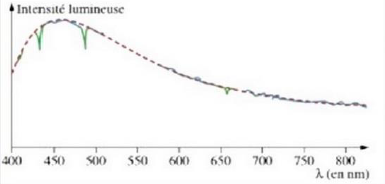
\includegraphics[width=0.5\columnwidth]{images/Exo1_Profil_Spectral_Etoile_Riga}
\end{center}
\caption{\label{fig:Profil_Spectral_Etoile_Riga}
Profil spectral de l'étoile de Riga}\end{figure}

\vspace{0.3cm}

\textbf{Document $2$}

\begin{figure}[h]
\begin{center}
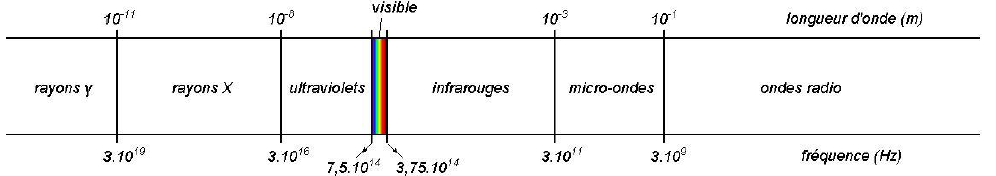
\includegraphics[width=\columnwidth]{images/Exo1_Spectre_Rayonnements_EM}
\end{center}
\caption{\label{fig:Spectre_Rayonnements_EM}
Spectre des rayonnements électromagnétiques}\end{figure}

\vspace{0.3cm}

\textbf{Document $3$ : loi de Wien}

\vspace{0.3cm}

La loi de Wien s'applique aux sources chaudes (aussi appelées corps noirs) et permet de relier la température $T$ d'une source chaude à la longueur d'onde de l'intensité maximale $\lambda_{max}$. La loi de Wien peut s'écrire sous forme de la formule suivante:

$$T = \frac{2.89 \times 10^{-3}}{\lambda_{max}}$$

avec $T$ en Kelvin ($\kelvin$), $\lambda_{max}$ en mètre ($\meter$), et la constante en Kelvin.mètre ($\kelvin.\meter$).

\vspace{0.3cm}

Le lien entre degré Celsius et Kelvin est donné par la relation: $\Theta(\celsius) = T - 273.15$.

\vspace{0.3cm}

\textbf{Document $4$ :} quelques détails sur les lampes halogènes:

\vspace{0.3cm}

En faisant passer un courant électrique dans le filament d'une ampoule, la température du filament s'élève: la couleur de la lumière émise par cette ampoule dépend alors de la température du filament.\newline
Les lampes halogènes contiennent un filament au tungstène chauffé à $3200$ \kelvin : une température plus élevée que dans les ampoules à filament classique. Ainsi la lumière fournie par une ampoule halogène est plus blanche et donne un meilleur rendu des couleurs, mais émet aussi des UV. C'est pourquoi une ampoule
halogène a toujours un verre de protection qui absorbe les UV.\newline
L'inconvénient des sources thermiques est qu'une grosse partie de l'énergie électrique n'est pas utilisée
pour produire de la lumière, mais de la chaleur.

%\vspace{0.3cm}

\newpage

A l'aide des documents ci-dessus et de vos connaissances, répondre aux questions suivantes:

\begin{enumerate}
\item Compléter le tableau ci-dessous (à reproduire sur la copie) en justifiant les résultats de la première ligne.

\begin{center}
\begin{tabular}{|c|c|c|c|}
\hline
Objet & $\lambda_{max}$ & $\Theta$ & Domaine du spectre \\
\hline
Corps humain &      &       &       \\
\hline
Etoile Riga &       &       &       \\
\hline
Lampe d'ambiance rouge  &       &       &   \\
\hline
Lampe halogène  &       &       &       \\
\hline
\end{tabular}
\end{center}

\item Donner la définition des grandeurs intervenant dans la loi de Wien.

\item On peut trouver la loi de Wien avec la formule $\lambda_{max} T = 2.89 \times 10^{6}$. Expliquer. Quelle est alors l'unité de $\lambda_{max}$ et de $2.89 \times 10^{6}$ ?

\item \begin{enumerate}[label=(\alph*)]
\item En utilisant la loi de Wien, expliquer comment évolue la longueur d'onde du maximum d'intensité en fonction de la température du corps chaud.
\item Justifier alors la phrase "la lumière fournie par une ampoule halogène est plus blanche […], mais émet
des UV" du document $4$.
\end{enumerate}

\end{enumerate}

\vspace{0.3cm}